\documentclass{article}
\input{WebMacros}
\input{SMacros}

\usepackage{graphicx}
\usepackage{times}
\usepackage{fullpage}

\usepackage{comment}

%\def\includegraphics#1{\texttt{#1}}

%\usepackage{listings}

\title{Solutions for Homework 2}
\author{Duncan Temple Lang}
\begin{document}
\maketitle

The ``solutions'' presented here are not intended to be a model
report, but rather to illustrate some of the things you might look at
and learn about R.

\begin{description}
\item[Q 1] 

  Let's start with a version that takes as input a matrix of
  parameters and vector of probabilities giving the proportions for
  which to sample each component.  The length of the vector should be
  the same as the number of rows as the matrix of parameters.
  We'll specify two here.
\begin{verbatim}
M1 = matrix( c(0, 1, 0.1,
              10, 2, 0.3,
              -5, 1, 0.1,
               25, 2 ,0.3,
              -50, 5, 0.2), 
            nrow = 5, ncol = 3, byrow = TRUE,
            dimnames=list(seq(1:5),c("Mean","SD","Prob")))


M2 = matrix(c( -6, 1.5,
                0, 1.5,
                6, 1.5), , 2, byrow = TRUE)
\end{verbatim}

  Now, before we go any further, I'd like to look at the densities.
  So, let's create a function that computes the density of the mixture
  at one or more values.  The following is one way to do it.  It
  accepts the probability vector and the parameter matrix of means and
  SDs for the mixture components, and the positions of $X$ at which to
  evaluate the density.  Then, it evaluates the density for each
  component at those points and adds them together using the
  proportions given in the vector \Svariable{p}.
\begin{verbatim}
dNormalMixture <-
function(x, p, params)
{
  tmp = cbind(params, p)

  rowSums(apply(tmp, 1, 
                  function(param) 
                     dnorm(x, param[1], param[2]) * param[3]))
}
\end{verbatim}
The actual implementation takes a short-cut: it adds the probability
vector as an extra column of the parameter matrix and then loops
over the rows, calling \SFunction{dnorm} for those values of x and
the specific parameters.  Adding the probabilities to the matrix
makes them available in each row.

Another way to do this is
\begin{verbatim}
dNormalMixture <-
function(x, p, params)
{
 rowSums(sapply(1:length(p),
                function(i)
                    dnorm(x, params[i, 1], params[i, 2]) * p[i]))
}
\end{verbatim}

You can now visualize the density of a mixture, e.g.
\begin{verbatim}
curve(dNormalMixture(x, rep(1/3, 3), M2),
        -12, 12, ylab = "density")
\end{verbatim}
and
\begin{verbatim}
curve(dNormalMixture(x, c(.2, .5, .1, .1, .1), M1), 
           -65, 35, xlab = "density")
\end{verbatim}
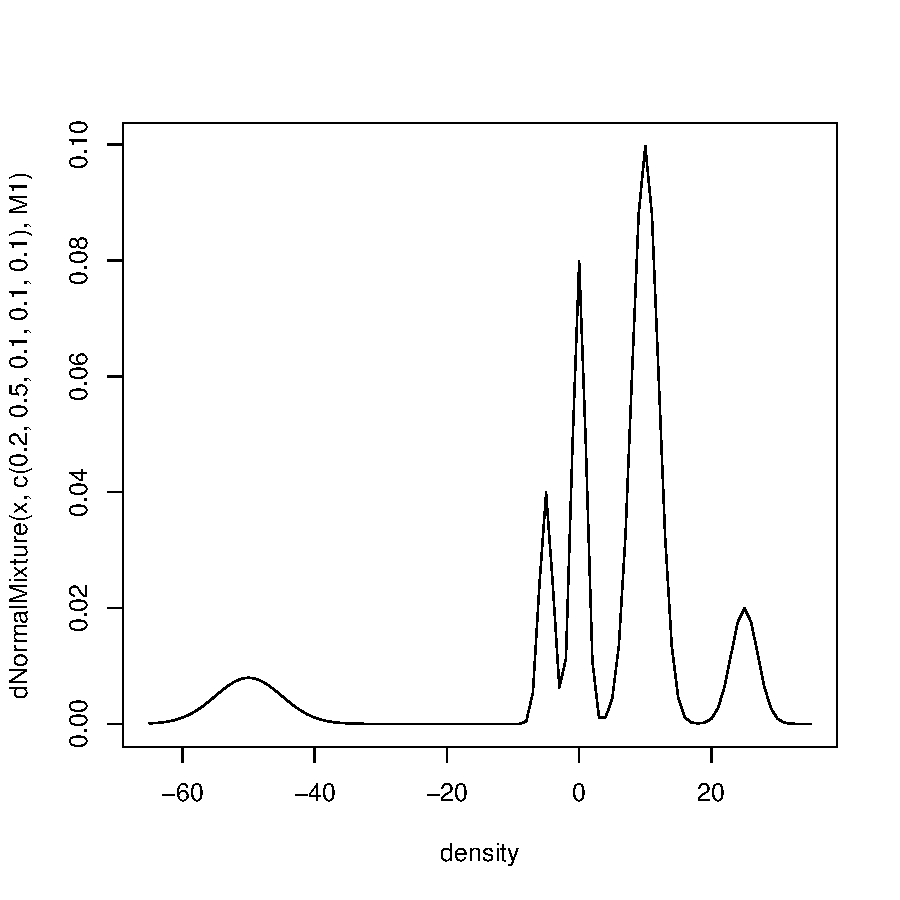
\includegraphics{images/mixtureDensity.pdf}


Let's now write a simple version of the function to generate
$n$ values from a general mixture of Normals.
Again, the important parameters are $n$, the number of values to
sample, $p$ the probability of selecting each of the components, and
the matrix of parameters for the components.  The mechanism we are
going to use is to generate a sample of size $n$ which identify from
which component to sample a Normal deviate.  When we have this vector
length $n$, we can loop over it and generate a single value from that
component of the mixture.  I've add two additional arguments to the
function definition below.  These are \SArg{whichComponent} and
\SArg{addComponentNames}.  The first of these allows the user to
explicitly specify the vector of component identifiers to sample for
each value. This has a default value which generates the sample if the
user does not specify it.  The reason we provide this is so that we
can explicitly control how many values to sample from each component.
This is useful when debugging, as we shall see.  The other argument --
\SArg{addComponentNames} -- merely instructs the code whether it
should identify which component was used to generate each value by
putting the index of the component as the element for that name.

\begin{verbatim}
normalMixture <-
function(n, p, params,
         whichComponent = sample(1:length(p), n, replace = TRUE, prob = p),
         addComponentNames = TRUE)
{
  ans <- sapply(whichComponent,
                 function(i) {
                    par = params[i,]
                    rnorm(1, par[1], par[2])
                 })

  if(addComponentNames)
     names(ans) <- whichComponent

  ans
}
\end{verbatim}
Hopefully the code should be reasonably self-explanatory given the
description above.

We can call it now with
\begin{verbatim}
x = normalMixture(10000, c(.3, .5, .2), M2)
\end{verbatim}
To verify that it is working, let's draw a histogram and superimpose
the  density.
\begin{verbatim}
hist(x, prob = TRUE, ylim = c(0, .14))
curve(function(x) dNormalMixture(x, c(.3, .5, .2), M2), 
       -12, 12, add = TRUE, col = "red")
\end{verbatim}
(We got the limits for the y-axis by trial and error.)

We should also try this for a different set of mixture inputs.
\begin{verbatim}
x = normalMixture(10000, c(.1, .2, .3, .2 , .2), M1)
hist(x, prob = TRUE, ylim = c(0, .15))
curve(dNormalMixture(x, c(.1, .2, .3, .2, .2), M1), 
       -60, 35, add = TRUE, col = "red")
\end{verbatim}

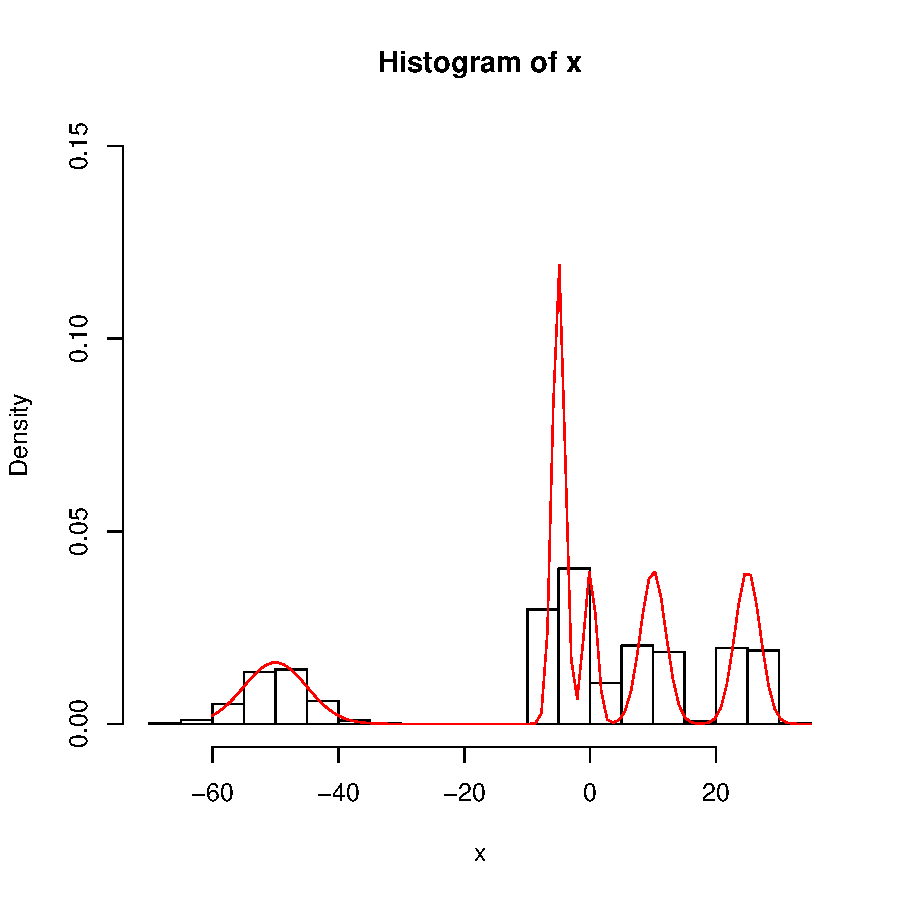
\includegraphics{images/mixtureSample1.pdf}

The shapes of the histograms are reasonably
consistent with the density curves, although
we probably need to either generate more
points or have a larger number of bins to get a better
visual fit.
\begin{verbatim}
hist(x, prob = TRUE, ylim = c(0, .15), breaks = 40)
curve(dNormalMixture(x, c(.1, .2, .3, .2, .2), M1), 
       -60, 35, add = TRUE, col = "red")
\end{verbatim}
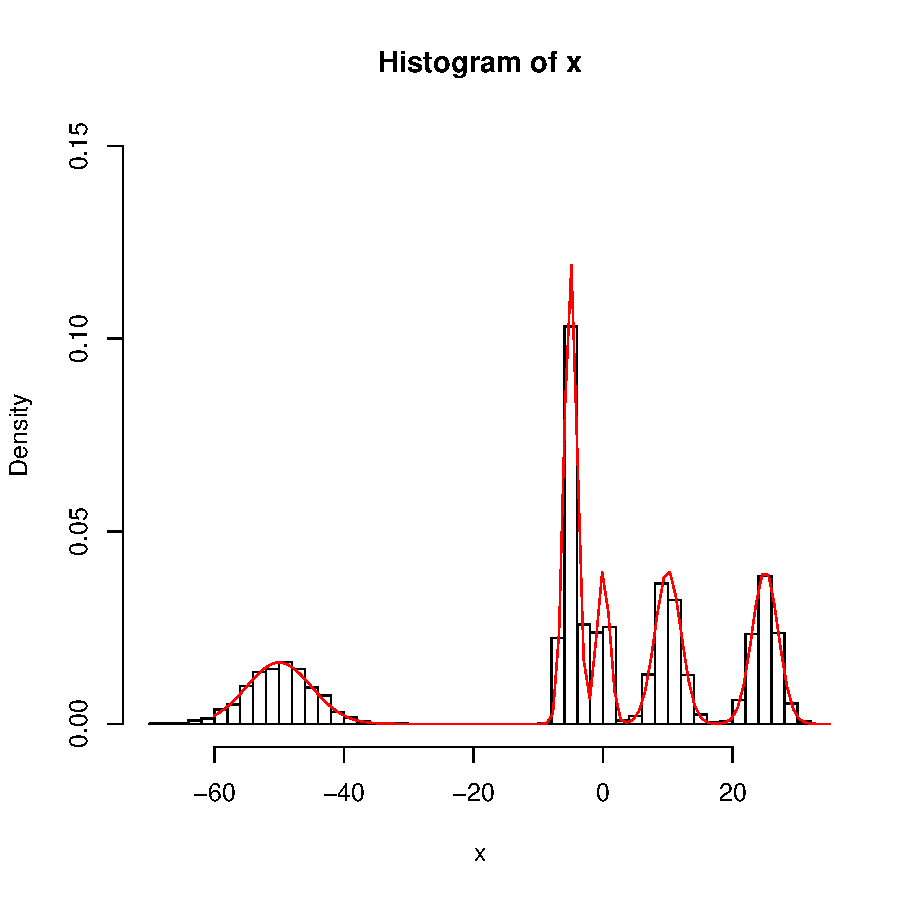
\includegraphics{images/mixtureSample1a.pdf}

Now, let's write the second and hopefully faster version of the
\SFunction{normalMixture} function.  In this version, we essentially
determine how many values -- $n_i$ --- we should sample from each
component $i$ and then generate that number in a single call to
\SFunction{rnorm}.  There are two ways to generate these counts for
each component. One is to take a sample as we did above of size $n$
from the set 1, 2, $\ldots$, k and then use \SFunction{table} to
compute the counts in each category/component.  Alternatively, we can
use \SFunction{rmultinom} to generate a single sample of $n$ values
from a multinomial distribution.
For example, 
\begin{verbatim}
rmultinom(1, 10, c(.2, .5, .3))
     [,1]
[1,]    0
[2,]    7
[3,]    3
\end{verbatim}
divides 10 into 3 groups with the corresponding probabilities of each
element being in that group.

Note that the first component had no values but was listed
in the answer.
Using \SFunction{table}, this does not happen.
For example, 
\begin{verbatim}
table(sample(1:3, 10, replace = TRUE, prob = c(.01, .5, .49)))
2 3 
5 5 
\end{verbatim}
has no entry for 1.
This difference makes the how we sample from the components
just a little different for the two approaches.

The idea is quite simple for \SFunction{rmultinom}.
We get the counts for the components and loop
over these and generate the $n_i$ values.
We need to index both the counts vector and 
the parameter matrix rows.
So we loop over the row indices
with \Sexpression{seq(along = counts)}
which is equivalent to \Sexpression{1:length(counts)}
but works well when counts has no elements.
\begin{verbatim}
normalMixture.faster <-
function(n, p, params)
{

  counts <- rmultinom(1, n, p)

   # loop over 1:length(p) and generate n_i values from 
   # each component.
  l = lapply(seq(along = counts),
              function(i) {
                 rnorm(counts[i], params[i, 1], params[i, 2])
              }) 

  unlist(l)
}
\end{verbatim}
Note that at the end of the \SFunction{lapply} call, we end up with a
list and we don't want to simplify it with \SFunction{sapply}. This is
because each element in the list will typically have different size.
So at the end of the function we call \SFunction{unlist} to unravel
all the values into a single vector.

The version using \SFunction{sample} and \SFunction{table}
is similar and given by
\begin{verbatim}
normalMixture.faster <-
  #
  #  The faster way to generate n values from a mixture
  #  by counting the number in each group and then 
  #  generating that number for each group in a single call.
  #
  #
function(n, p, params, 
          counts = table(sample(1:length(p), n, replace = TRUE, prob = p)),
          addNames = TRUE)
{
  ans <- unlist(lapply(seq(along = counts),
                 function(id) {
                   par = params[as.integer(names(counts)[id]),]
                   rnorm(counts[id], par[1], par[2])
                 }))

  if(addNames)
     names(ans) <- rep(names(counts), counts)

  ans
}
\end{verbatim}
The primary differences between here and the one above is that we have
added the extra arguments \SArg{counts} and \SArg{addComponentNames}
as we did earlier.  And the loop in the \SFunction{lapply} has to do
some apparently more complex indexing to get the parameters for the
particular parameter.  This is because the position in the
\Svariable{counts} variable does not necessarily correspond to the row
of the component in parameter matrix. This is because some of the
categories may have no elements and be dropped from the frequency
table.  So we turn the name of the element of \Svariable{count} from a
string to a row index in the parameter matrix.  Again, we add names to
identify the component if they are requested.

Again, we want to check the histograms as above.  (Do this!)  In
addition to this check, however, we can also compare the output from
each function to each other.  We can use a Q-Q plot for this since the
two distributions of numbers are supposed to be the same.

\begin{verbatim}
x1 = normalMixture(10000, c(.1, .2, .3, .2 , .2), M1)
x2 = normalMixture.faster(10000, c(.1, .2, .3, .2 , .2), M1)
qqplot(x1, x2)
\end{verbatim}
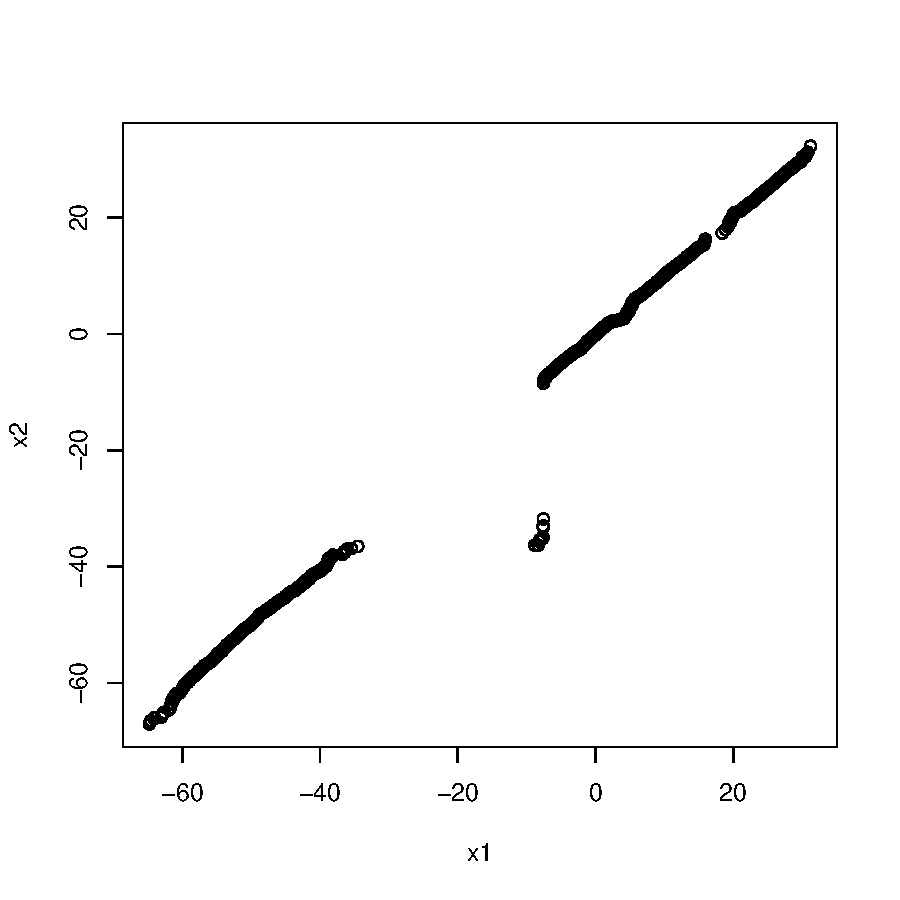
\includegraphics{images/algorithmBasicQQplot.pdf}

This is supposed to yield a straight line up to sampling variability.
And with $10,000$ observations, it should be very good.  However, we
see major departures from the line.  The primary trend is definitely a
straight line as we expect, but there are major ``bumps''.  After a
bit of investigation, we can figure out what is causing these and why
the Q-Q plot appears erroneous. And then we can conclude that the
algorithms are really giving qualitatively similar results.

Let's take a look at the actual values coming from each algorithm.  We
want to add these to the Q-Q plot and it would be good to color code
them base on which component they were sampled from.  To do this, we
need to be able to determine the component for each value.  This is
what the \SArg{addComponentNames} argument does in our two functions;
it adds the component identifiers as names for the  result vector, 
identifying each element's component.
The function \SFunction{showQQ} and \SFunction{drawRug} below 
draws the Q-Q plot with this additional information.
\begin{verbatim}
showQQ =
  #
  # Draws a QQ plot of the two data vectors
  # and assumes they have names identifying
  #
function(x, xx, pch = "o", showLine = TRUE)
{  
  qqplot(x, xx, pch = pch, pty = "s") # force square aspect ratio.
  if(showLine)
     abline(a = 0, b = 1, col = "red")

  drawRug(x)
  drawRug(xx, 3)
  drawRug(xx, 2)
}

drawRug =
  #
  # Plot the data for the different groups identified by their names.
  #
function(x, side = 1) {
       k = levels(factor(names(x)))
       colors = rainbow(length(k))
       for(i in seq(along = k))
         rug(x[names(x) == k[i]],  col = colors[i], side = side)
}
\end{verbatim}

Now, we can use this to see more information about our plot.
\begin{verbatim}
showQQ(x1, x2)
\end{verbatim}
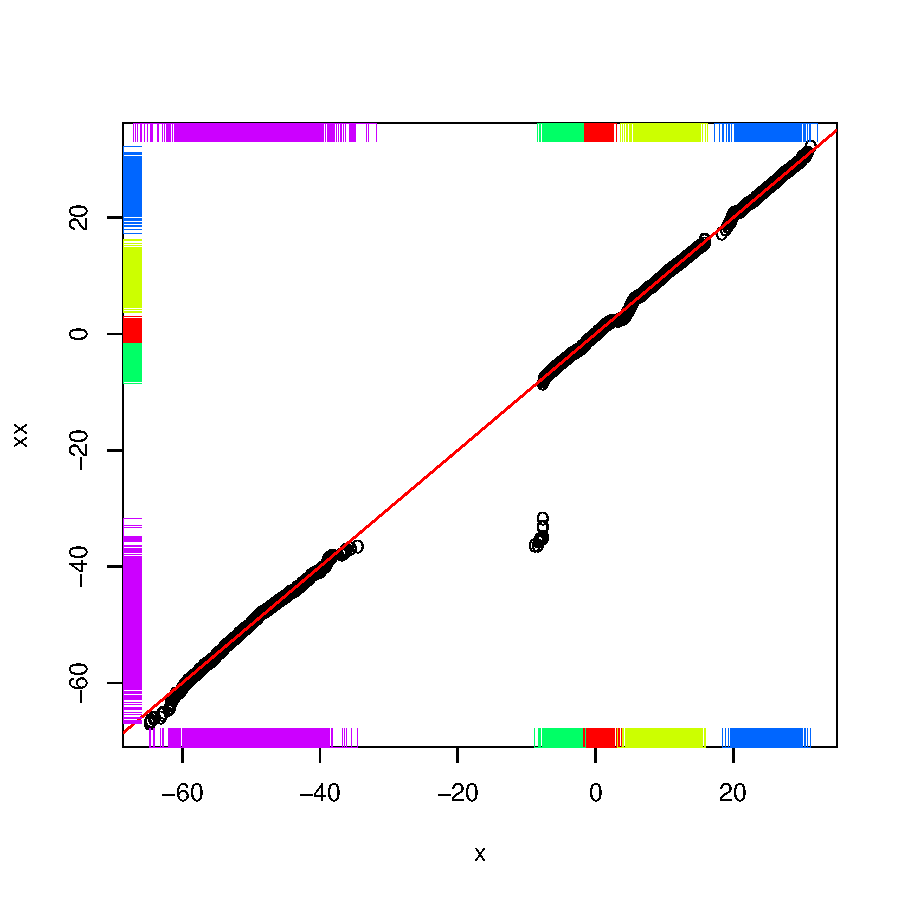
\includegraphics{images/algorithmRugQQ.pdf}

Hopefully, you can see that the bumps occur at the break points
between two components, on either the horizontal or vertical axis.
Specifically, look at the lower-left corner of the plot.  There is a
big departure from the line, with a couple of points below and to the
right of the line.  If we see which components these correspond to, we
see what is the problem.  On the horizontal axis, these points are
from the second component (green), but on the vertical axis, they are
from the first component (purple).  Since these two components have
very different typical values, the minimum of the second is nowhere
close to the maximum of the first.  And so the pairs of points are way
off the straight line we expected.  This is good explanation of why
the bumps appear.  It also tells us that the problem is that because
of the randomness in the sampling process, there are fewer
observations from component 1 in the first set of data
(\Svariable{x1}) than in \Svariable{x2}.  It is this difference that
really causes the bumps.  If we force them to have the same number in
each component, then we should get a Q-Q plot much closer to the
expected straight line.  We can do this by specifying which components
to sample from in each algorithm using the \SArg{which Component}
argument I added to my versions of the functions.

\begin{verbatim}
components = sample(1:5, 10000, prob = c(.1, .2, .3, .2 , .2), replace = TRUE)
x1 = normalMixture(10000, c(.1, .2, .3, .2 , .2), M1,
                         whichDist = components)
x2 = normalMixture.faster(10000, c(.1, .2, .3, .2 , .2), M1,
                           counts = table(components))
\end{verbatim}
Now, the Q-Q plot of these two vectors is a straight line,
with  breaks where there are no values.

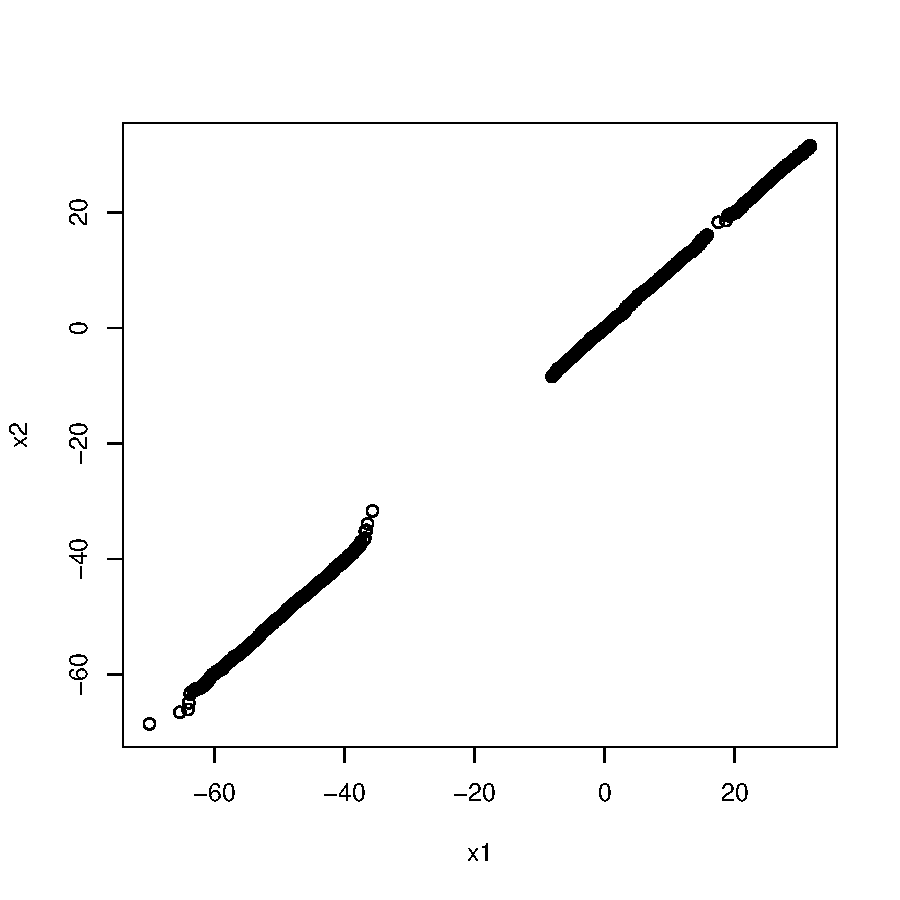
\includegraphics{images/SimpleQQEqualCount.pdf}

Using \SFunction{showQQ}, we can see that the components match up
in this case and there are no bumps.

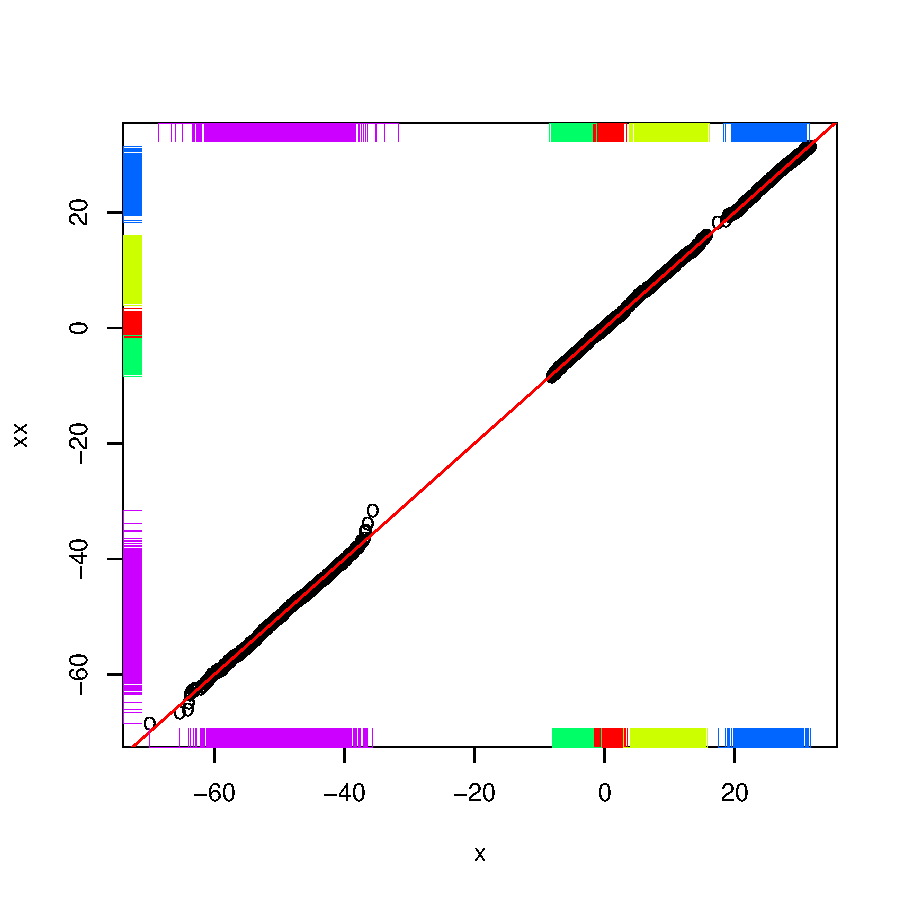
\includegraphics{images/QQEqualCount.pdf}

Now, we can move on to comparing the speed of the two algorithms for
different sample sizes.  We will look at this for $5$ different sample
sizes, $1, 10, 100, 1000, 10000$.  Then we loop over the two functions
and for each of these, we loop over the sample sizes.
Then, for each sample size and function pair, we perform the
random sample $11$ times and count the time for each.
\begin{verbatim}

# Can do this in two separate pieces of code, but really a repetition.
# and if one needs to change one, then need to change the other.
# e.g. adding system.time.
sampleSizes <- c(1, 10, 100, 1000, 10000)
names(sampleSizes) <- sampleSizes

# Choose prime numbers (2, 5, 11) so that we can identify the
#  dimensions in the result if they are collapsed.

tt <- lapply(list(basic = normalMixture,
                   counts = normalMixture.faster),
        function(f) {
              lapply(sampleSizes,
                      function(n) {
                         sapply(1:11, function(i) {
                            system.time(f(n, c(.3, .2, .5), 
                                          matrix(c(.2, .1, 
                                                   .5, .3, 
                                                   .8, 1), ,
                                                  2, byrow = TRUE)))
                       })
                     })
             })



# Note that this doesn't work in S-Plus as n is not in 
# the scope of the inner function.

 # Just look at elapsed time.
elapsedTimes <- sapply(tt, function(f)  
                            sapply(f, function(m) mean(m[3, drop = FALSE])))

matplot(sampleSizes, elapsedTimes, type = "l",
            xlab = "Sample Size", ylab = "seconds", 
            main = "Elapsed time for two algorithms")

legend(400, .9*max(elapsedTimes), c("basic", "counts"), 
        col = 1:2, pch = as.character(1:2))
\end{verbatim}
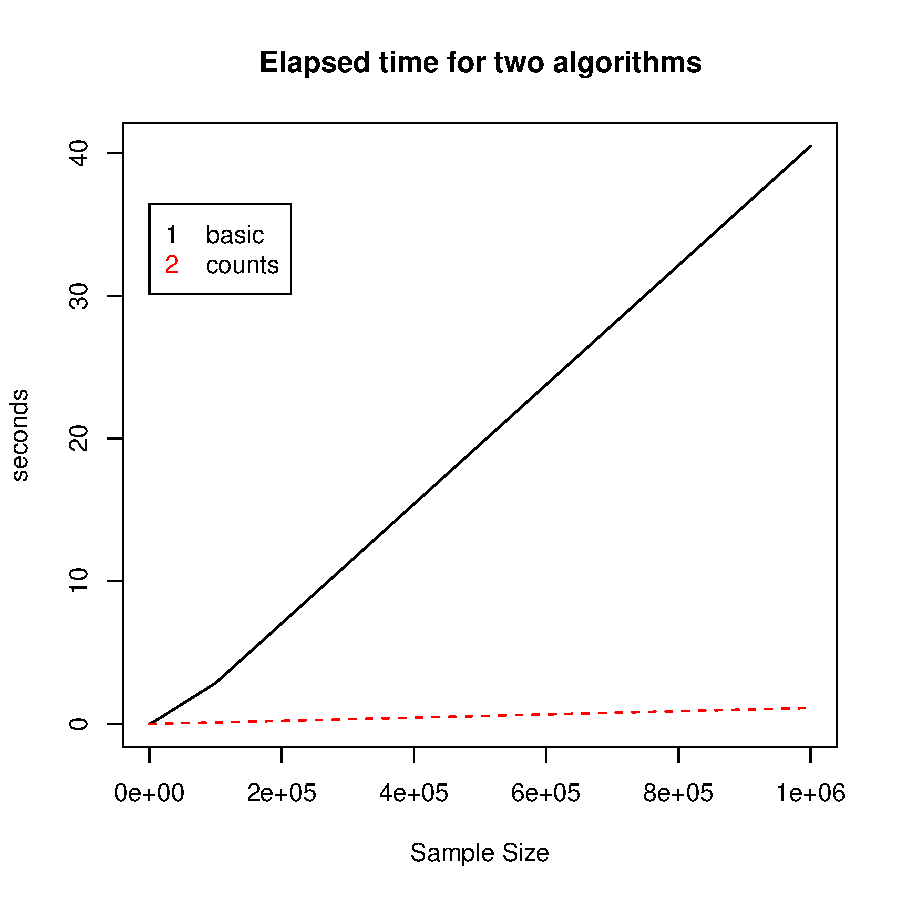
\includegraphics{images/algorithmTimes.pdf}
We see that there is a large difference in run-times as $n$ increases.
The second algorithm is much faster.
As we go to larger $n$

Any oddity for $n = 1$ is caused by the fact that we cannot measure
very short runs accurately. Rather than taking the mean of
$k$ runs for $n = 1$, we should take the total time
for $k$ runs and divide it by $k$ when the time being measured
is very small.


The moral to take away from this exercise is that the naive way of
doing things is a good one to work on first and use as a validation
test; but it is often appropriate to find a vectorized form of the
function in order to make it more efficient, but only if the time
spent making the code faster is less than the amount of time saved in
running the more efficient code!


\item[Acceptance Rejection Sampling]

This is a relatively straightforward application of
acceptance-rejection (AR) sampling.  It is hard to find a majorizing
density $g(x, y)$, so we use a simple 2-dimensional uniform.

We will generate pairs $(x, y)$ from this 2-dimensional uniform by
generating $x$ and then $y$ from separate, independent uniform
distributions. In this case, both $X$ and $Y$ have the same
distribution, namely $U(0, 100)$.

For a given $(x, y)$ pair, we accept it if a random value from $U(0,
c')$ is less than $f(x, y)$, i.e. the density $f$ evaluated at the
potentially acceptable point.  All we need is to find the value of
$c'$ to complete the algorithm.  The value $c'$ satisfies $c' =
c\times g(x, y)$ for which $c' \ge f(x, y)$ for all $(x, y) \in
[0,100] \times [0, 100]$, i.e. that majorizes our density of interest.
Since $g(x, y)$, our 2-dimensional uniform, is constant, we are
concerned with its value, just the value for which $c' \ge f(x, y)$
for all $(x, y)$ pairs of interest.

To determine $c'$, we need to find the maximum value of $f(x, y)$.  We
cannot do this analytically without looking at the definition of $f(x,
y)$ in the \SFunction{nodeDensity} function. Even then, it may be hard
or impossible to solve exactly.  Instead, we can evaluate $f(x, y)$ at
many points on a grid of $(x, y)$ pairs and then look at the regions
at which the maxima occur.  For each of these potential maximum
points, we can break the neighborhood into grids of finer resolution
and continue to iteratively search for the maximum, getting
increasingly closer to the true answers.

Since we are only looking for a majorizing function rather than the
exact maximum, we can find the sample maximum and use a slightly
higher value.  Adding this ``fudge'' factor will just make our
acceptance/rejection mechanism slightly less efficient.

To find the maximum, we can use
\SFunction{outer} again.
\begin{verbatim}
x = seq(0, 100)
z = outer(x, x, nodeDensity)
max(z)
\end{verbatim}

The maximum is $ 3.983295$.
To zoom in on the neighborhoods,
we need to find out where the maxima occur.
\begin{verbatim}
r = x[row(z)[ z == max(z)]]
c = x[col(z)[ z == max(z)]]
\end{verbatim}
And these give us 
the pairs
$(61, 1)$ and $(1, 61)$.
Let's look at the region $[0, 2] \times [60, 62]$
\begin{verbatim}
x = seq(0, 2, length = 100)
y = seq(60, 62, length = 100)
z = outer(x, y, nodeDensity)
max(z)
\end{verbatim}
We get $3.983565$.  So we did find a slightly bigger value, but it is
likely that a value of $c' = 3.99$ will work well.

We can also take some protective measures in our code.  If we evaluate
$f(x, y)$ and find a value greater than $c'$, we will issue a
warning. Of course, it will be too late if we are already using random
values generated from this algorithm, but it is still a useful check
point.  We can even modify the algorithm to use the largest value of
$c'$ that it has encountered.


The following is a very simple and slow version of the
acceptance-rejection sampling approach for the problem.
\begin{verbatim}
rDensity.slow = function(n = 100, c.prime = 3.99)  {
  if(n > 1)
    return(replicate(n, rDensity(1)))

  while(TRUE) {
     pos = runif(2, 0, 100)
     f = nodeDensity(pos[1], pos[2])
     if(runif(1, 0, c.prime) < f)
       return(pos)
   }
}
\end{verbatim}
What this does is to accept a request for $n$ observations from the
density function \SFunction{nodeDensity}.  However, the function works
on just one observation at a time. So it calls itself $n$ times.  When
it is called with $n = 1$, it goes ahead and uses the AR approach.  It
continues indefinitely until it finds an acceptable point $(x, y)$.
It generates a target pair $(x, y)$ by sampling 2 observations from a
$U(0, 100)$, thus giving $x$ and $y$.  Then it evaluates $f(x, y)$ and
then compares this to a random observation from $U(0, c')$.  If it is
acceptable, the pair is returned; otherwise, it continues and
generates a new pair and checks that.


We can check that this does indeed give us $n$ pairs of $(x, y)$.
\begin{verbatim}
p = rDensity(10)
\end{verbatim}
We should check that they are all within the right range, i.e. $[0,
100]$.

How can we  determine whether the values come from that
density?
One approach is to take a large sample and count the number
in different bins.
\begin{verbatim}
p = rDensity(1000000)
x = seq(0, 100)
obs = table(cut(p[, 1], x), cut(p[,2], x))
\end{verbatim}
We can plot these counts as a function of 
X and Y.
\begin{verbatim}
x = seq(.5, length = 100)
persp(x, x, obs, theta = 30, phi = 30)
\end{verbatim}

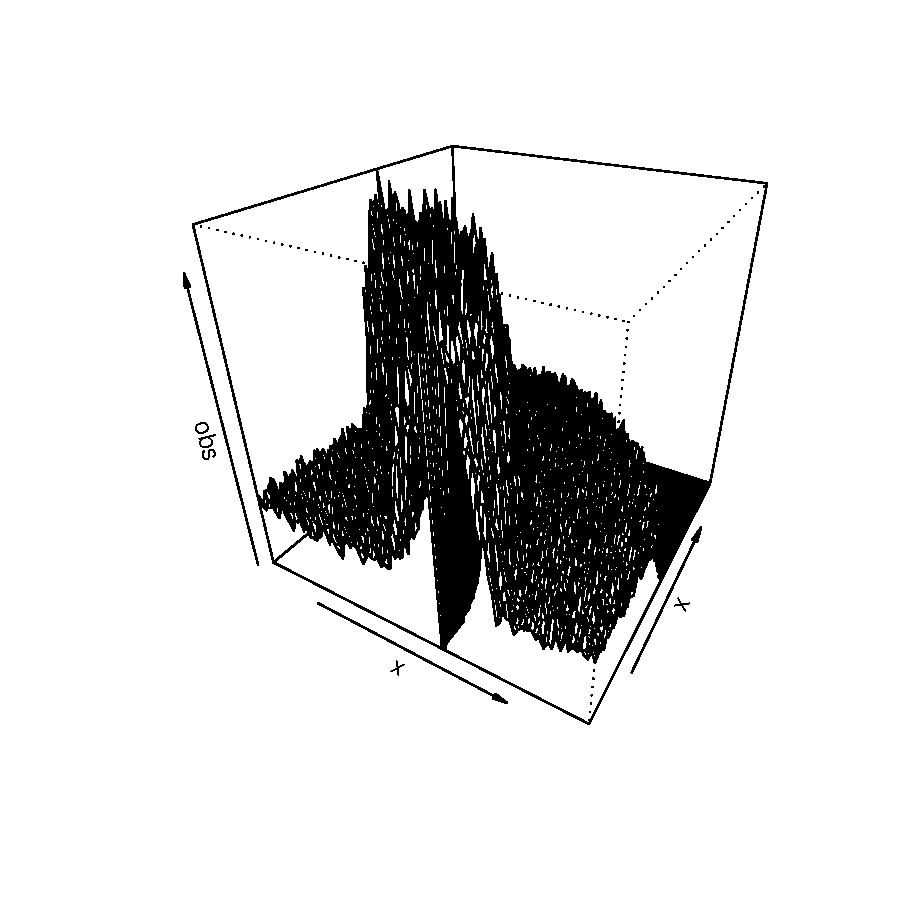
\includegraphics{images/nodeDensitySample.pdf}


Alternatively, we can draw the actual density
(as before) and then superimpose the scaled
counts:
\begin{verbatim}
v = persp(x, x, outer(x, x, nodeDensity), phi = 30, theta = 30)
g = expand.grid(x, x)
oo = as.integer(obs)
points(trans3d(g[,1], g[,2], 4*oo/max(oo), v), col = "red", pch = "+")
\end{verbatim}
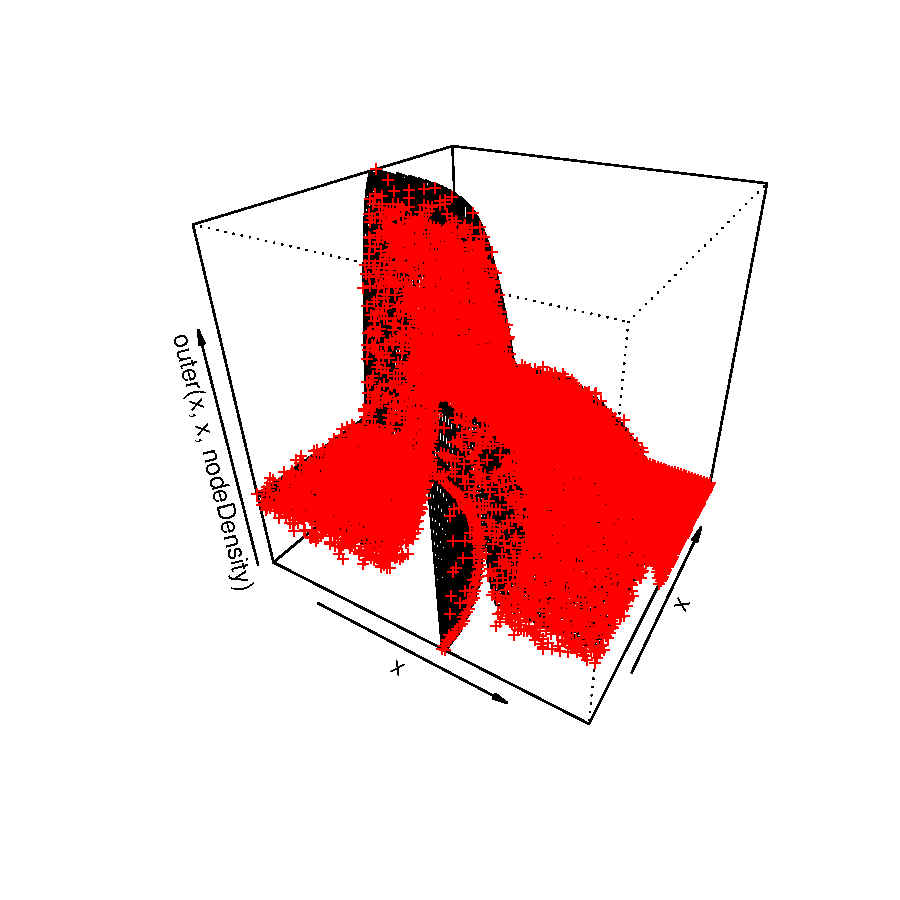
\includegraphics{images/nodeDensityPoints.pdf}
It is hard to see how good a fit this is.


We can compare the observed counts in each bin to the expected number
in each bin.  The expected number can be approximated by the average
$f(x, y)$ within the bin multiplied by the total number, i.e.
\Sexpression{nrow(p)}.
\begin{verbatim}
x = seq(.5, length = 100)
expected = outer(x, x, nodeDensity) * nrow(p)
\end{verbatim}
Of course, this approximation only works well when 
$f(x,y)$ is reasonably constant within a bin.
This is clearly not true for the high ridges.


We can also compute marginal and conditional distributions.  For $y =
0$, we should see the density being close to the front slice of the 2-D
density in the perspective plot:
\begin{verbatim}
curve(nodeDensity(x, rep(0, length(x))), 0, 100, n = 10000)
points(seq(.5, length = 100), as.numeric(4*obs[,1]/max(obs[, 1])), col = "red")
\end{verbatim}
We can do this for arbitrary $y$
with the command
\begin{verbatim}
curve(nodeDensity(x, rep(y, length(x))), 0, 100, n = 10000)
points(seq(.5, length = 100), as.numeric(4*obs[,as.integer(y)]/max(obs[, 1])), col = "red")
\end{verbatim}


Let's return to examining our function.  Note that we call
\SFunction{runif} for each pair $(x, y)$ and again for each $u$ to
determine if we accept the point.  The random number generation
functions in R can return $n$ values in a single call and this is much
more efficient than $n$ calls each returning a single observation.  We
can use this idea to make our function faster.  Firstly, we will try
to generate lots of values in a single step.  We will reject some, so
we will return and generate however many more are needed in the
subsequent attempts.  Each time, the number we need to generate should
be decreasing.  And in each iteration, we are generating numerous
values, not just a single value. So we are taking advantage of the
vectorized operations.

In addition to this speedup, we can also do a generic ``trick'' for
acceptance-rejection sampling.  Since we expect to reject some
proportion of the generated observations, we will generate more than
we need in the hope of getting the right number.  When asked for $n$
values, we generate $n' = k \times n$ values where $k > 1$.  By
carefully choosing $k$ (by theoretical or empirical reasoning), we can
find a trade-off between generating too many and not generating
enough.


A revised version of the function now looks like the following.
We create an empty answer object which is a matrix with 2 columns
and no rows! We will add our acceptable observations as we generate
them.
We increase the number we will generate by multiplying by
the user-specifiable \SArg{factor}.
In our case, for every observation we want, we will generate 3.

We then enter our acceptance-rejection loop,
continuing to sample until we have enough
observations.
For each iteration, we generate
\Svariable{nmore} candidate points.
Then we evaluate $f(x, y)$ at these points.
Then, we find out which are acceptable by generating
\Svariable{nmore} values from $U(0, c')$.
Note that we take advantage of the speed up here
of generating many values from this one distribution.
If we were not using a constant majorizing density, we
would not be able to do this. Instead, we would have
to generate each value from $U(0, c \times g(x, y))$.

Having determined the acceptable points, we append these to the answer
matrix. If the resulting matrix has $n$ or more rows, we can finish,
so we break from the loop.  Otherwise, we need to generate additional
observations and we need \Sexpression{n - row(ans)} of them.  So
again, we ask for \SArg{factor} times that many to take into account
the expected number of rejections.

At the end, we make certain to return only the first $n$ rows of the
answer matrix. If the caller asked for $n$, we must not give them back
$> n$ observations.

\begin{verbatim}
rDensity =
function(n = 100, factor = 2.9, c.prime = 3.99)
{
   # Create an empty answer matrix with zero rows.
  ans = matrix(NA, 0, 2)

   # Determine how many we need to generate to get
   # the n that we want. 
  nmore = ceiling(factor*n)

   # This will store the proportion that were accepted each iteration.
  rate <- numeric(0)
  
  while(TRUE) {
     pos = matrix(runif(2*nmore, 0, 100), ncol = 2)
     f = nodeDensity(pos[,1], pos[,2])
     
     acc = (runif(nmore, 0, c.prime) < f)
     ans <- rbind(ans, pos[acc,])

     rate[as.character(nmore)] <- sum(acc)/nmore
     
     if(nrow(ans) >= n)
        break

     nmore =  ceiling(factor * (n - nrow(ans)))
   }

   # Limit the result to just the first n rows
   # in case we ended up with more accepted.
   ans = ans[1:n,]

   # Put the rate information on the object
   attr(ans, "rate") <- rate
   ans
}

\end{verbatim}


Note that when we asked for $n$ values, we got back 
a matrix as expected, but there was also an attribute
named \SArg{rate} attached to it which we can access
as 
\begin{verbatim}
z = rDensity(100)
attr(z, "rate")
\end{verbatim}
This is a named vector.  Each element tells us what proportion of the
generate candidate points were accepted.  The name for that element
tells us how many candidate points there were.  This information tells
us the empirical probability of acceptance.  We can use this to
calibrate the function.  These are essentially estimates of $p$, the
probability of acceptance.  The variance of the estimate is $ \hat{p}
(1 - \hat{p})/n_i$, where $n_i$ is the number of items being sampled
of which $\hat{p}$ are rejected.  So we would want to take a weighted
average of these by using 1 over the variance as the weight.  And the
variance is essentially then 1 over the number of items that were up
for acceptance or rejection since $p$ is assumed to be the same.  So
the weights are 
\begin{verbatim}
w = as.integer(names(attr(z, "rate")))
w = w/sum(w)
\end{verbatim}
and our estimate is 
\begin{verbatim}
sum(attr(z, "rate")* w)
\end{verbatim}

At the end of each run of this function, we could update the default
value of the \SArg{factor} argument.  If our function had its own
environment, the updated estimate would be easy to store in the
environment.

Similarly, since we evaluate $f(x, y)$ many times, we can verify that
the values are all less than \SArg{c.prime}.  If we find one that
isn't, we can update the default value of \SArg{c.prime} to that newly
found maximum.  Again, if the function has its own environment, this
is easy to do.

The following code gives us what we want.
\begin{verbatim}
rDensity =
function(n = 100, factor = 1/accRate, c.prime = maxDensity)
{
   # Create an empty answer matrix with zero rows.
  ans = matrix(NA, 0, 2)

   # Determine how many we need to generate to get
   # the n that we want. 
  nmore = ceiling(factor*n)

   # This will store 
  rate <- numeric(0)
  
  while(TRUE) {
     pos = matrix(runif(2*nmore, 0, 100), ncol = 2)
     f = nodeDensity(pos[,1], pos[,2])
     
     m = max(f)
     if(m > c.prime) { 
       warning("new maximum value for density found in rDensity. Check previous output!")
       maxDensity <<- m
     }

     acc = (runif(nmore, 0, c.prime) < f)
     ans <- rbind(ans, pos[acc,])

     rate[as.character(nmore)] <- sum(acc)/nmore
     
     if(nrow(ans) >= n)
        break

     nmore =  ceiling(factor * (n - nrow(ans)))
   }

   # Limit the result to just the first n rows
   # in case we ended up with more accepted.
   ans = ans[1:n,]

   # Put the rate information on the object
   attr(ans, "rate") <- rate

    # Now update the acceptance rate estimate.
   rate <- structure(c(accRate, rate), names = c(names(accRate), names(rate)))
   n =  sum(as.integer(names(rate)))
   w = as.integer(names(rate))/ n
   accRate <<- sum(w * rate)
   names(accRate) <<- as.character(n)
  browser()

   ans
}
environment(rDensity) <- new.env()
environment(rDensity)$maxDensity <- 3.99
environment(rDensity)$accRate <- c("1000" = 1/2.9)
\end{verbatim}

So this version is self-correcting and converges to the appropriate factor.
(Check the details.)


\item[Bootstrap]
We start by fitting a linear model to each of the two subsets
within the data, that is the first $4000$ observations for
device A, and the remaining $6000$ for device B.
\begin{verbatim}
fit.A = lm(y ~ x,  devices, subset = device == "A")
fit.B = lm(y ~ x,  devices, subset = device == "B")
\end{verbatim}
Take a look at the coefficients from each
and look at the summary.
\begin{verbatim}
summary(fit.A)

Call:
lm(formula = y ~ x, data = devices[devices$device == "A", ])

Residuals:
      Min        1Q    Median        3Q       Max 
-36.01996  -2.93127   0.01089   2.73319  31.93671 

Coefficients:
            Estimate Std. Error t value Pr(>|t|)    
(Intercept)  2.50767    0.78471   3.196  0.00141 ** 
x            7.38950    0.06252 118.194  < 2e-16 ***
---
Signif. codes:  0 '***' 0.001 '**' 0.01 '*' 0.05 '.' 0.1 ' ' 1 

Residual standard error: 5.79 on 3998 degrees of freedom
Multiple R-Squared: 0.7775,     Adjusted R-squared: 0.7774 
F-statistic: 1.397e+04 on 1 and 3998 DF,  p-value: < 2.2e-1

> summary(fit.B)
summary(fit.B)

Call:
lm(formula = y ~ x, data = devices, subset = device == "B")

Residuals:
     Min       1Q   Median       3Q      Max 
-73.6386  -7.0776  -0.2027   6.6787  73.2976 

Coefficients:
            Estimate Std. Error t value Pr(>|t|)    
(Intercept)   3.3512     1.5734    2.13   0.0332 *  
x             7.3296     0.1251   58.58   <2e-16 ***
---
Signif. codes:  0 '***' 0.001 '**' 0.01 '*' 0.05 '.' 0.1 ' ' 1 

Residual standard error: 13.99 on 5998 degrees of freedom
Multiple R-Squared: 0.3639,     Adjusted R-squared: 0.3638 
F-statistic:  3431 on 1 and 5998 DF,  p-value: < 2.2e-16 
\end{verbatim}

Note that the range of the residuals is quite different, but most
importantly, the coefficients are different.  However, the Standard
Error is quite large so they are not significantly different from each
other. However, they are supposed to be the same.


A plot of the residuals against $y$ for device B yields a strange
result.  And the correlation is high.
\begin{verbatim}
cor(resid(fit.A), devices$y[devices$device == "A"])
[1] 0.472
\end{verbatim}

We now have two sets of residuals.
Let's compute their variances
\begin{verbatim}
evar.A = var(resid(fit.A))
evar.B = var(resid(fit.B))
\end{verbatim}
Now, let's compute the single linear fit 
for both devices together but by weighting the
observations by the inverse of the variances of the
errors. We put the weights into the original data frame
for convenience in using them later and associating them
with residuals.
\begin{verbatim}
devices$weights <- c(rep(1/evar.A, 4000), rep(1/evar.B, 6000))
\end{verbatim}
The fit is then
\begin{verbatim}
fit = lm(y ~ x, devices, weight = weights)
\end{verbatim}
Again, let's look at the summary.
\begin{verbatim}
summary(fit)

Call:
lm(formula = y ~ x, data = devices, weights = weights)

Residuals:
      Min        1Q    Median        3Q       Max 
-6.229151 -0.503896 -0.005983  0.477158  5.509459 

Coefficients:
            Estimate Std. Error t value Pr(>|t|)    
(Intercept)  2.67411    0.70214   3.808 0.000141 ***
x            7.37771    0.05592 131.931  < 2e-16 ***
---
Signif. codes:  0 '***' 0.001 '**' 0.01 '*' 0.05 '.' 0.1 ' ' 1 

Residual standard error: 1 on 9998 degrees of freedom
Multiple R-Squared: 0.6352,     Adjusted R-squared: 0.6351 
F-statistic: 1.741e+04 on 1 and 9998 DF,  p-value: < 2.2e-16 
\end{verbatim}

Let me tell you at this point that the model truly is linear and the
errors are from two double exponential distributions.  The
coefficients are $\beta_0 = 2.45$ and $\beta_1 = 7.39$.  The scale
parameters for the Double exponentials are $.25$ and $.1$ for device A
and B respectively.  (The variance of the double exponential is
related inversely to the scale parameter, so small values of $\theta$
lead to greater variability.)

So we see that the estimates of the coefficients are not too bad and
generally improved from the fit on device B alone.


Let's put the residuals from this fit into the data frame
so that we can use them in the non-parametric bootstrap in
part b).
\begin{verbatim}
devices$residuals <- residuals(fit)
\end{verbatim}


In each bootstrap regime that we consider in a), b), and c), the only
difference is how we generate the bootstrap sample.  After we have the
new bootstrap sample, we fit the model and get the coefficient
estimates.

\begin{enumerate}
\item[a)] The code for this is quite simple.  Let's keep the
  proportions for device A and B the same as in the original sample.
  We will therefore take a random sample with replacement of the
  observations from device A and then a separate sample with
  replacement from the $6000$ observations for device B.
For each of the $B$ bootstrap samples, we do
\begin{verbatim}
rows <- c(sample(1:4000, 4000, replace = TRUE),
          sample(1:6000, 6000, replace = TRUE) + 6000)

beta.star <- coef(lm(y ~ x, devices, weights = weights, subset = rows))
\end{verbatim}

So our code is
\begin{verbatim}
beta.star <-
 replicate(B, 
           coef(lm(y ~ x, devices, weights = weights, 
                subset = c(sample(1:4000, 4000, replace = TRUE),
                           sample(1:6000, 6000, replace = TRUE) + 6000))))
\end{verbatim}

The result is \Svariable{beta.star} which is a $2 \times  99$ matrix.
The summary statistics are
\begin{verbatim}
rowMeans(beta.star)
rowMeans(beta.star)
(Intercept)           x 
   2.509937    7.391906 
\end{verbatim}
The Standard Deviations are given by
\begin{verbatim}
apply(beta.star, 1,sd)
(Intercept)           x 
 0.64259112  0.05215145 
\end{verbatim}

We have $99$ observations for each coefficient
and so we can compute marginal confidence intervals
for each parameter separately.
\begin{verbatim}
apply(beta.star, 1, quantile, c(0.025, .975))
      (Intercept)        x
2.5%     1.482661 7.281707
97.5%    3.887659 7.474910
\end{verbatim}
There is a lot of variability in the intercept. The
slope parameter is much more precisely estimated.
We can also compare this to the confidence interval
given from the overall weighted fit based on Normal
approximation theory ($n = 10,000$):
\begin{verbatim}
7.37771 + 1.96*c(-0.05592, 0.05592)
[1] 7.268107 7.487313
\end{verbatim}
This is wider than our bootstrap interval.


\item[b)] In this bootstrap, we generate our bootstrap datasets by
  sampling a collection of X's and using the coefficients from our
  original overall weighted fit -- \Svariable{coef(fit)} -- to compute
  $E[Y^*] = X^*\hat\beta$. Then we add residuals sampled at random
  from the residuals of our overall weighted fit.
  Since we want to use weighted least squares again, we sample both
  the residual and its weight.  Also, we will preserve the number of 
  observations from device A and device B.
So our code is
\begin{verbatim}
beta.star.b <-
 replicate(B,
    {
     x.star <- devices$x[c(sample(1:4000, 4000, replace = TRUE),
                           sample(1:6000, 6000, replace = TRUE) +  6000)]

     ids <-  c(sample(1:4000, 4000, replace = TRUE),
               sample(1:6000, 6000, replace = TRUE) +  6000)
     y.star <- coef(fit)[1] + coef(fit)[2]*x.star + devices$residuals[ids]

     coef(lm(y.star ~ x.star, weights = devices$weights[ids]))
    })
\end{verbatim}

Again, we have a $2 \times 99$ matrix.
And we can look at the summaries.
\begin{verbatim}
rowMeans(beta.star.b)
(Intercept)      x.star 
   2.582711    7.384019 
\end{verbatim}
And a $95\%$ confidence interval is computed as
\begin{verbatim}
apply(beta.star.b, 1, quantile, c(0.025, .975))
      (Intercept)   x.star
2.5%     1.201687 7.292582
97.5%    3.728896 7.496088
\end{verbatim}


\item[c)] The final version is to estimate $\theta_A$ and $\theta_B$
  and then generate residuals from the distributions with these
  parameters, rather than using the residuals from the
  \Svariable{fit}.  The Maximum Likelihood Estimate for $\theta$, the
  scale parameter, in a Double Exponential for a sample
  $x_1, \ldots, x_n$ is given by
  $$\hat\theta = \frac{n}{\sum_i^n | x_i |}$$
  Now, we can estimate $\theta_A$ and $\theta_B$ in R as
\begin{verbatim}
theta.A = 4000/sum(abs(devices$residuals[devices$device == "A"]))
theta.B = 6000/sum(abs(devices$residuals[devices$device == "B"]))
\end{verbatim}
This gives $0.243$ and $0.101$ respectively.  These are very close to
the true values.

We can generate observations from a double exponential with centrality
parameter 0 and scale parameter $\theta$ using the following function:
\begin{verbatim}
rDoubleExp <-
function(n, theta = 1)
{
  sample(c(-1, 1), n, replace = TRUE) * rexp(n, theta)
}  
\end{verbatim}
This just generates $n$ values from a regular exponential parameter
with parameter $\theta$. Then we multiply this by $1$ or $-1$ with 
probability $.5$, giving the double exponential distribution.


To generate the parametric bootstrap sample, using the double
exponential distribution, we use the following code
that modifies that in part b):
\begin{verbatim}
beta.star.c <-
 replicate(B,
    {
     x.star <- devices$x[c(sample(1:4000, 4000, replace = TRUE),
                           sample(1:6000, 6000, replace = TRUE) +  6000)]

     y.star <- coef(fit)[1] + coef(fit)[2]*x.star + 
                    c(rDoubleExp(4000, theta.A), rDoubleExp(6000, theta.B))

     coef(lm(y.star ~ x.star, weights = devices$weights))
    })
\end{verbatim}
Again, we end up with a $2 \times 99$ matrix.
Means are given by
\begin{verbatim}
rowMeans(beta.star.c)
(Intercept)      x.star 
   2.614283    7.382756 
\end{verbatim}
And confidence intervals given by
\begin{verbatim}
apply(beta.star.c, 1, quantile, c(0.025, .975))
      (Intercept)   x.star
2.5%     1.010563 7.229525
97.5%    4.465705 7.511029
\end{verbatim}

The variability is larger here. Yet, given that this is how the model
was actually generated, this is most accurate.  So it is not a small
CI that we want, but an accurate one.  Note that in practice we would
chose one based on a real understanding of the data and the random
process at work. We do not chose the one that is most convenient
for our interpretation!
\end{enumerate}

Since we are exploring the behavior of the bootstrap,
we can compare our three sets of results.
Let's compare the distributions of the intercepts 
for the three bootstrap methods.
\begin{verbatim}
boxplot(list(a = beta.star[1,], b = beta.star.b[1,], c = beta.star.c[1,]))
\end{verbatim}
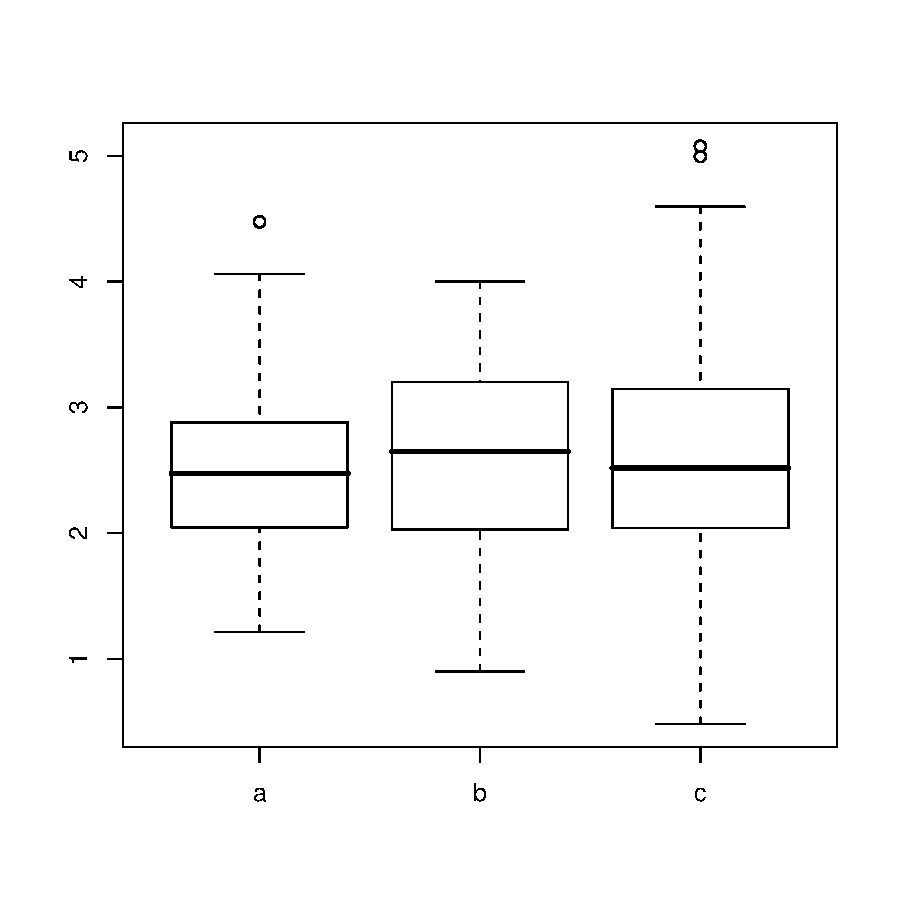
\includegraphics{images/bootstrapIntercepts.pdf}

Similarly, the distributions of the intercepts are seen
in
\begin{verbatim}
boxplot(list(a = beta.star[2,], b = beta.star.b[2,], c = beta.star.c[2,]))
\end{verbatim}
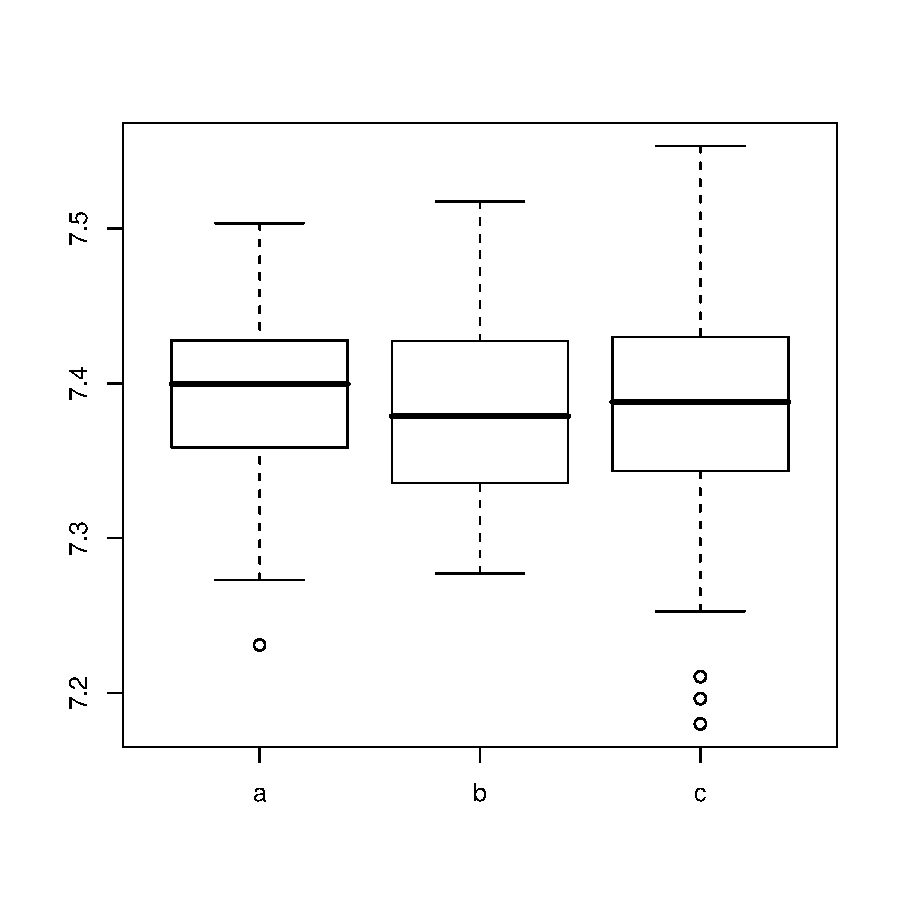
\includegraphics{images/bootstrapSlopes.pdf}

We see that in both plots, the medians are similar, but that the
spread is larger as we go from a to b to c.

Of course, for each bootstrap sample, we have a pair $(\hat\beta_0^*,
\hat\beta_1^*)$.  So we can plot $\hat\beta_0^*$ against
$\hat\beta_1^*$ and identify which pair is from which 
bootstrap method -- a, b, or c.

\begin{verbatim}
matplot(cbind(beta.star[1,], beta.star.b[1,], beta.star.c[1,]), 
        cbind(beta.star[2,], beta.star.b[2,], beta.star.c[2,]), 
        pch = c("o", "+", "*"), 
        col = c("blue", "green", "red"),
        xlab = "Bootstrap intercept",
        ylab = "Bootstrap slope", cex = 2)
\end{verbatim}
We can add marginal confidence intervals for each parameter for
each bootstrap approach.
\begin{verbatim}
# Draw the confidence intervals for each parameter for each bootstrap
#  approach
star = list(beta.star, beta.star.b, beta.star.c)
colors = c("blue", "green", "red")
sapply(seq(along = star),
       function(i) {
            # compute the quantiles
        q = apply(star[[i]], 1, quantile, c(0.025, .975))
        for(j in 1:2) {
          if(j == 1) 
            lines(q[,j], rep(7.175 + i/100, 2), col = colors[i])
          else
            lines(rep(.5 + i/10, 2), q[,j],col = colors[i])
        }
            
      })
\end{verbatim}

And we can also superimpose the convex hull -- the smallest polygon
containing all the points -- for each bootstrap distribution.
\begin{verbatim}
# Convex hulls of the distributions.
polygon(t(beta.star[, chull(beta.star[1,], beta.star[2,])]), border = "blue")
polygon(t(beta.star.b[, chull(beta.star.b[1,], beta.star.b[2,])]), border = "green" )
polygon(t(beta.star.c[, chull(beta.star.c[1,], beta.star.c[2,])]), border = "red")
\end{verbatim}
We also add the Normal confidence interval.
\begin{verbatim}
s = summary(fit)$coefficients
lines(c(s[1,1]  -1.96* s[1,2], s[1,1] + 1.96* s[1,2]), rep(7.170, 2))
lines(rep(.5, 2), c(s[2,1]  -1.96* s[2,2], s[2, 1] + 1.96* s[2,2]))
\end{verbatim}

And lastly we add a legend
\begin{verbatim}
legend(3, 7.5, paste(c("a", "b", "c", "Normal", ), c("0", "+", "*", "")),
          text.col = c("blue", "green", "red", "black"))
\end{verbatim}

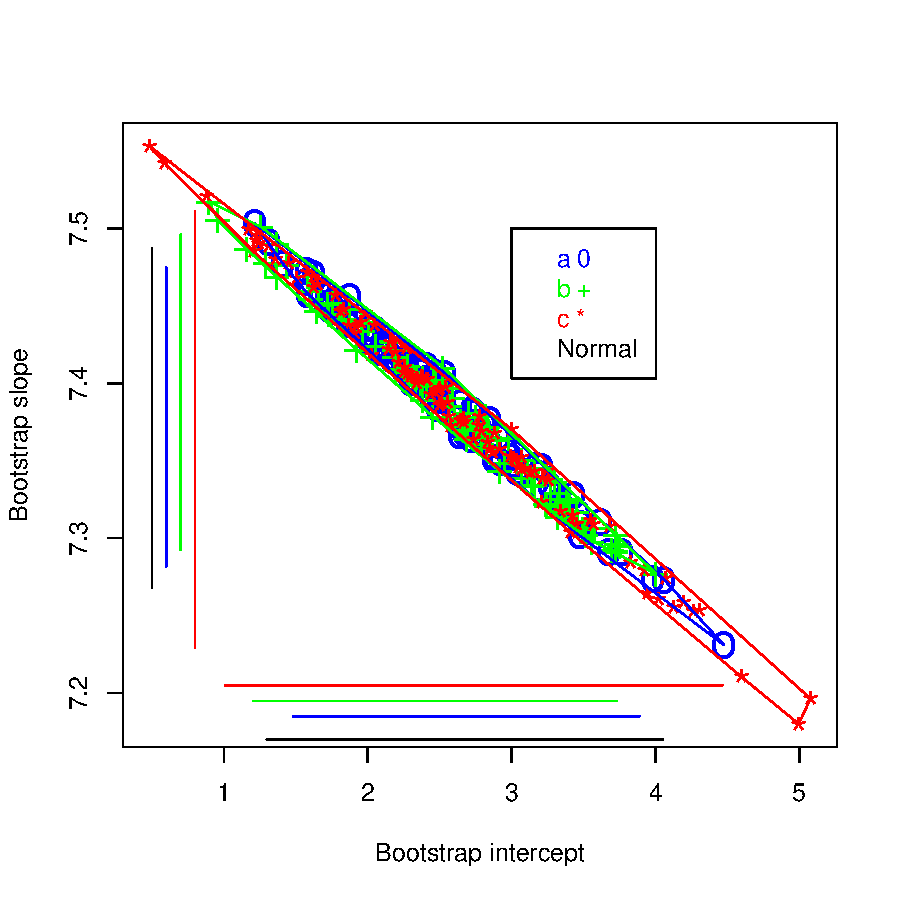
\includegraphics{images/BootstrapsCIs.pdf}

We note that the coefficient estimates are highly correlated.  Large
values of the intercept are associated with small values of the slope
and vice verse.

Again, we see that the last bootstrap technique (the red one) in fact
gives rise to the largest intervals.  It is bigger than the Normal
which is the black line.  So we see that the bootstrap has given us
different and in this case more accurate confidence intervals.  And we
have seen that the form of the bootstrap sample generation matters. We
need to know what the underlying process is.

\end{description}

\end{document}
